\documentclass[t]{beamer}


%useful packages
\usepackage{color,soul}
\usepackage{amsmath,amsthm,amscd,amssymb,bm}
\usepackage{hyperref}
\usepackage[utf8]{inputenc}
\usepackage{enumerate}
\usepackage{xcolor}


%personal definitions and commands
\newcommand{\R}{\mathbb{R}} 
\newcommand{\E}{\mathbb{E}}
\newcommand{\V}{\mathbb{V}}
\newcommand{\C}{\mathbb{C}}
\newcommand{\Prob}{\mathbb{P}}
\newcommand{\e}{\epsilon}
\newcommand\numberthis{\addtocounter{equation}{1}\tag{\theequation}} %allows numbering of single equations in align* environment
\newcommand{\mtx}[1]{\ensuremath{\bm{\mathit{#1}}}}
\newcommand{\B}{\hat{\boldsymbol{\beta}}}
\newcommand{\Cov}{\mathbb{C}\text{ov}}
\newcommand{\N}{\mathcal{N}}


% \usepackage{beamerthemesplit} // Activate for custom appearance

\title{Replication of `The Power of Forward Guidance Revisited'}
\author{}
\date{\today}

\begin{document}

\frame{\titlepage}



\begin{frame}
\frametitle{Outline}
\begin{enumerate}
\item Motivation
\item MNS's heterogenous agent NK model
\item Steady state
\item Dynamics: forward guidance
\end{enumerate}
\end{frame}

\frame{
\frametitle{Motivation}
\begin{itemize}
\item In the basic NKM, output/inflation response to forward guidance is implausibly large.
\item A potential reason is the complete markets assumption.
\pause
\item Is the output response to forward guidance smaller in a model with idiosyncratic income risk and incomplete markets?
\end{itemize}

}

\frame{

\frametitle{Forward guidance in the basic NKM}
Consider the plain vanilla NKM studied in class
\begin{align*}
y_t &= \E_t[y_{t+1}] - \sigma(i_t - \E_t[\pi_{t+1}] - r_t^n) &\text{ `NK IS curve'}\\
\pi_t  &= \beta\E_t[\pi_{t+1}]  + \kappa y_t &\text{ `NKPC'}
\end{align*}
\pause

with monetary policy rule:
\begin{align*}
r_t = i_t - \E_t[\pi_{t+1}] = r_t^n + \e_{t,t-j},
\end{align*}
where $\e_{t,t-j}$ is a monetary shock in period $t$ that is announced in period $t-j$.
}

\frame{

\frametitle{AIM implementation}
\begin{align*}
\tilde{r}_t &= a_1MA_t^1 + a_2MA_t^2 + a_2MA_t^3 + a_4MA_t^4 + a_5MA_t^5
\end{align*}
with
\begin{align*}
MA_t^1 &= \e_{t+5,t}=
\begin{cases}
1 &\text{ if } t=1 \\
0 &\text{ otherwise.}
\end{cases}
\end{align*} 
and
\begin{align*}
MA^j_t = MA_{t-1}^{j-1}
\end{align*}
and $a_1=a_2=a_3=a_4=0$, $a_5 = 1$
}


\frame{
\frametitle{Forward guidance in the basic NKM}
\begin{figure}
 \centering
    
        %\centering
        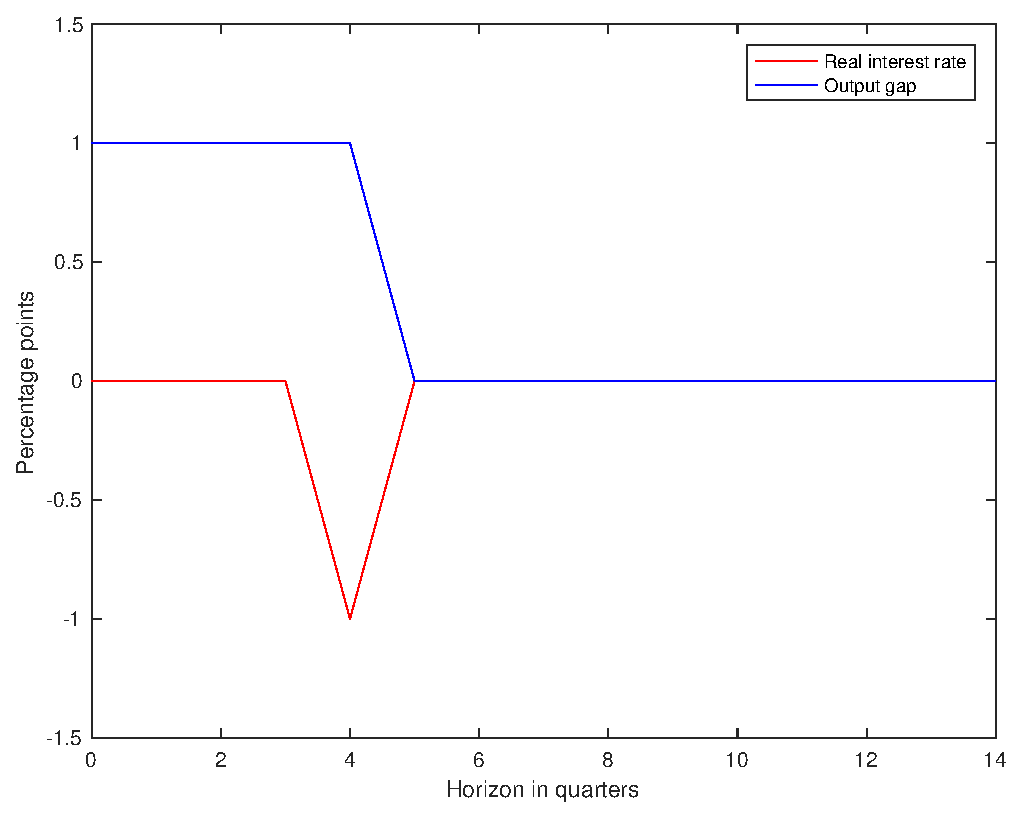
\includegraphics[width=0.8\textwidth]{IR_1_R.eps}


\end{figure}

}

\frame{
\frametitle{Forward guidance in the basic NKM}
Why is the output response so big?\vspace{1cm}

$\implies$ Euler equation ($\sigma=1$):
\begin{align*}
\E_t[\Delta\tilde{c}_{t+1}] = \beta \tilde{r}_t 
\end{align*}
\pause
No borrowing constraint $\implies$ agent takes full advantage of intertemporal substitution.
}

\frame{
\frametitle{MNS's HANK model}
\pause
Household's problem
\begin{align*}
&\max_{\{c,\ell, b_{t+1}\}} \E_0\sum_{t=0}^\infty \beta^t \left(\frac{c_{h,t}^{1-\gamma}}{1-\gamma} - \frac{\ell_{h,t}^{1+\psi}}{1+\psi}\right)\\
\\
&\text{s.t. } c_{h,t} + \frac{b_{h,t+1}}{1+r_t} = b_{h,t} + W_tz_{h,t}\ell_{h,t} - \tau_t\bar\tau(z_{h,t}) +D_t\\
\\
&\text{\& } b_{h,t+1} \geq 0.
\end{align*}
}

\frame{
\frametitle{Calibration}
$z_{h,t}$ follows a 3-point Markov chain with transition matrix
\begin{align*}
\bm{\Gamma} = 
\begin{bmatrix}
0.966 &	0.0338 &	0.00029 \\
0.017&	0.966& 	0.017 \\
0.0003 &	0.0337 &	0.966
\end{bmatrix}
\end{align*}
Other parameter values are standard.
}

\frame{
\frametitle{Solving for steady state}
\begin{itemize}
\item Solve for the household's policy function using the `endogenous grid method'.
\pause
\item Basic idea is to iterate on the Euler equation:
\begin{align*}
c^{-\gamma} = \beta(1+\bar r) \sum_{z'}\Pr(z'|z)(g^0(z',b'))^{-\gamma}
\end{align*}
and use the budget constraint to back out today's bond holdings.

\end{itemize}
}

\frame{
\frametitle{Solving for steady state}
\begin{enumerate}
\item Guess an initial level of s.s dividends and taxes $X^0 = [\bar D^0, \bar\tau^0]$.
\item Using this guess and other steady state prices, compute the HH's policy function.
\item Simulate the distribution of bond holdings, using the policy function.
\item Compute aggregate consumption, $\bar C^0$.
\item Compute the implied level of dividends and taxes consistent w/ mkt clearing, $\tilde X^0 = [\tilde{D}^0, \tilde{\tau}^0]$ 
\item Update the guess of dividends and taxes: $X^1 = \omega  \tilde{X}^0 + (1-\omega)X^0$. I set $\omega=0.5$.
\item Iterate until convergence: $X^n=X^{n-1}$.
\end{enumerate}

}
\frame{
\frametitle{Some results}
\begin{figure}
 \centering
    
        %\centering
        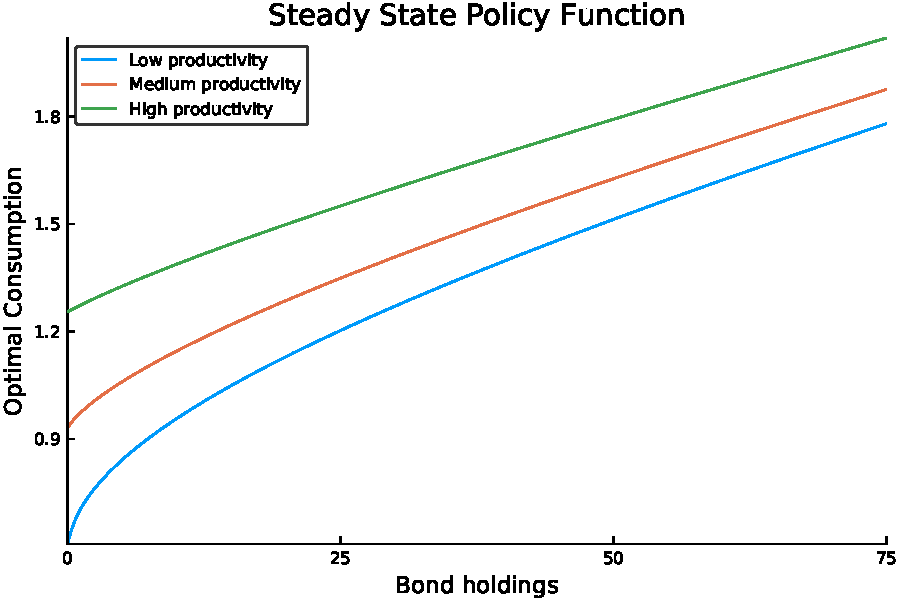
\includegraphics[width=1\textwidth]{pol_fn_C.pdf}


\end{figure}

}

\frame{
\frametitle{Some results}
\begin{figure}
 \centering
    
        %\centering
        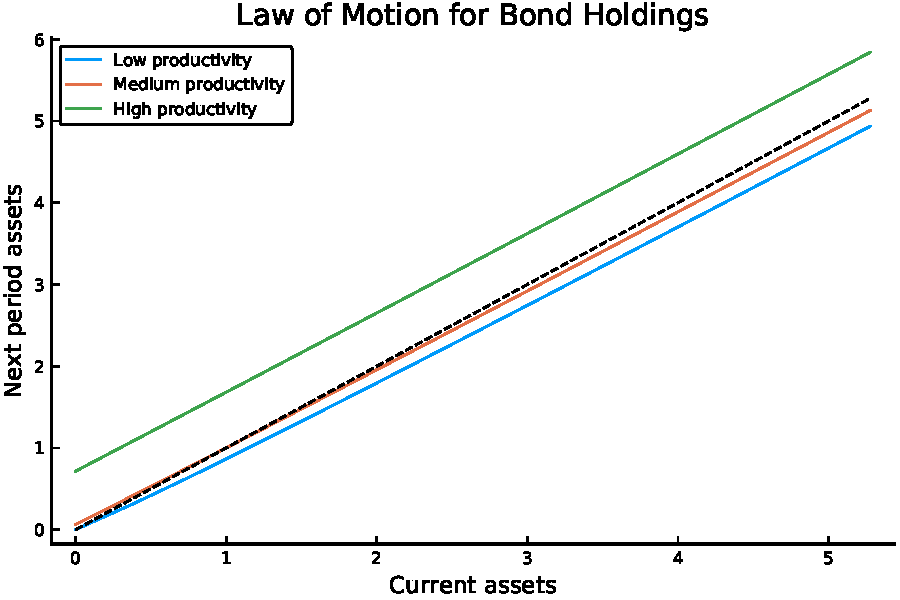
\includegraphics[width=1\textwidth]{pol_fn_B.pdf}


\end{figure}

}
\frame{
\frametitle{Some results}

\begin{figure}
 \centering
    
        %\centering
        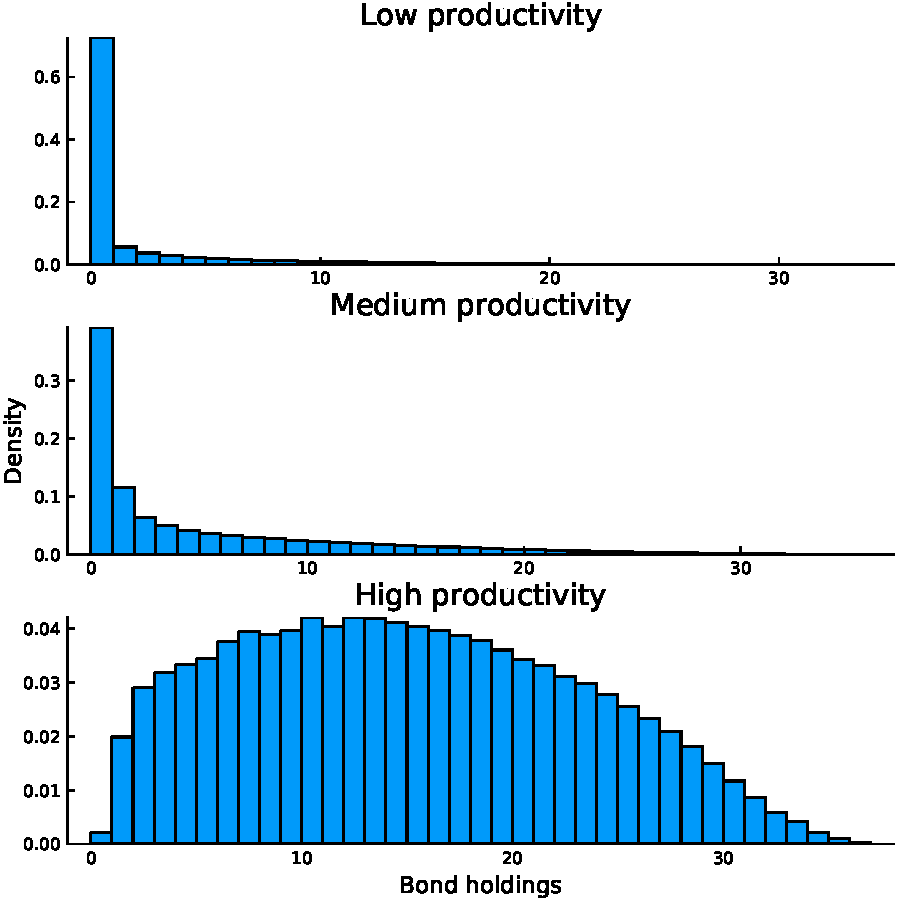
\includegraphics[width=0.7\textwidth]{bonds.pdf}


\end{figure}

}

\frame{
\frametitle{Problems with my `solution'}

}







\end{document}
